\documentclass{paper}

\usepackage{graphicx}

\title{Measurement of Energy Loss in the ADS FFAG Foil}
\author{Chris Rogers }

\begin{document}

\maketitle

\section{Data Taking}
The principle of the experiment is to measure the synchronous phase of the beam
as a function of RF voltage. When energy is "just" returned to the beam, the
sychronous phase should be 90$^{o}$.

Data was taken on the afternoon of Friday 4th April. The closed orbit correction 
magnet was set to  468 A. A closed orbit could not
be found for the more desirable setting of 700 A so this was not used. Two 
channels were chosen for readout; S12 and a pickup in the RF cavity. We decided
to readout many points to improve the measurement accuracy, so the scope was set
to $10^6$ points per trace, averaging over 128 ion source pulses.

Beam was injected over 6.6 us. There was some discussion on this  point, as 
there was a concern that this might cause some not-captured beam loss (which makes noise on 
the signal). In the end it was decided that the linac beam is bigger than the RF
bucket no matter what, so there would always be some not-captured beam loss; so
getting a bigger signal would be more helpful.

The following input signal voltages were used. Note that the pickup voltage is
measured, which is different to these voltages below.

\begin{itemize}
\item 2.5 V
\item 3.0 V
\item 2.0 V
\item 1.5 V
\item 1.0 V
\item 0.5 V
\end{itemize}

At this point the ion source was looking unwell so the ion source current was 
increased.The "bunch" signal in the beam monitor was examined dynamically. 
It was noted that there is a a bunch signal even with no RF, just coming from the beam 
circulating. An attempt was made to reduce this signal by chopping the front and 
back of the ion source pulse 
to see if it helps. It was then decided to take some more data at lower voltages.

\begin{itemize}
\item 1.2 V
\item 1.4 V
\item 1.6 V
\item 1.8 V
\end{itemize}

The data was stored as \verb|phis.tar.gz|.

\section{Data}
The analysis followed several stages. The time of the peaks in the RF signal and 
the bunch monitor signal S12 was calculated. The peak to peak time difference
was studied in each signal to understand the stability of the signal and then 
used to calculate RF frequency. The time difference between adjacent peaks of 
the two signals was then studied to identify beam capture behaviour. The peak to
peak voltage difference on the RF signal was used to calculate the RF voltage. 
The RF voltage was compared with the difference between time of RF signal and
beam signal, and the resulting relationship was used to infer an energy loss.

$10^6$ counts were read out, with time between counts of 0.2 ns. The data 
was recorded by averaging over 128 ion source pulses.

\subsection{Peak Finding Algorithm}
Peaks were found in the first instance by smoothing the data using a Gaussian
function with standard deviation 50 ns. This was followed by a search for peaks 
performed by looking for the peak values within a 50 ns window. The window was
advanced in steps of 25 ns and the peak value was recorded within the window. 
Peak values at the window edge were ignored.

This initial estimate was refined by fitting a quadratic function to the
data points in the region of the peak. The points used for fitting were 
dynamically selected by requiring that the residuals of the fit $x(fit)-x(data)$
should not have a standard deviation much larger than the estimated standard 
deviation of the data very close to the peak. The time and magnitude of the 
peak, $t_p, y_p$ were estimated from the fit parameters, according to
\begin{eqnarray}
y &=& a_0 + a_1 t + a_2 t^2 \\
t_p &=& -\frac{a_1}{2a_2}  \\
y_p &=& -\frac{a_1^2}{4a_2}+a_0
\end{eqnarray}
The errors were calculated using the standard relationship
\begin{eqnarray}
\mathbf{V}(t_p, y_p) = \mathbf{J} \mathbf{V}(\vec{a}) \mathbf{J^T}
\end{eqnarray}
where $\mathbf{V}$ are the covariance matrices. $\mathbf{V}(\vec{a})$ was 
calculated by taking the numerical derivative of the fit parameters with respect 
to the $\chi^2$, which is done  automatically by the ROOT software used for 
fitting. $\mathbf{J}$ is the Jacobian for $(t_p(\vec{a}), y_p(\vec{a}))$, given
by
\begin{equation}
\mathbf{J} = \left(\begin{array}{ccc}
    0 & -1/2a_2 & a_1/2a_2^2 \\
    1 & -a_1/2a_2 & a_1^2/4a_2^2
\end{array}\right)
\end{equation}

\subsection{RF Signal}
The RF signal was generated by means of a pick-up in the RF cavity which was 
read out by an oscilloscope. An example of the resultant trace is shown in
Fig. \ref{fig:signals}, along with the resultant beam monitor signal.

\begin{figure}
	\centering
		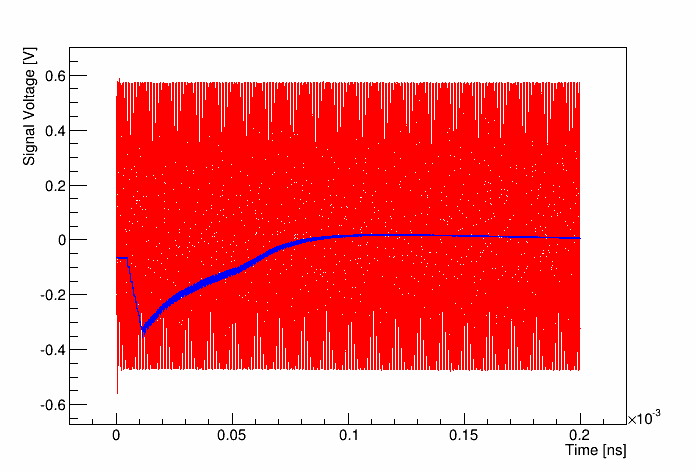
\includegraphics[width=\textwidth]{images/V=1_03_signals}
		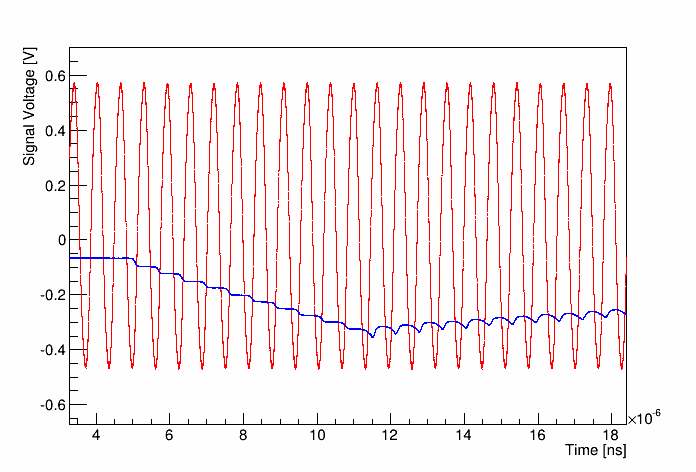
\includegraphics[width=\textwidth]{images/V=1_03_signals_zoom}
	\caption{Example of measured RF pickup and bunch monitor signals for RF peak 
           voltage of 0.5 volts. (Top) the full signal trace (Bottom) the 
           region around injection.
           The RF pickup trace is shown in red; the bunch monitor trace is shown
           in blue.}
	\label{fig:signals}
\end{figure}

\begin{figure}
	\centering
		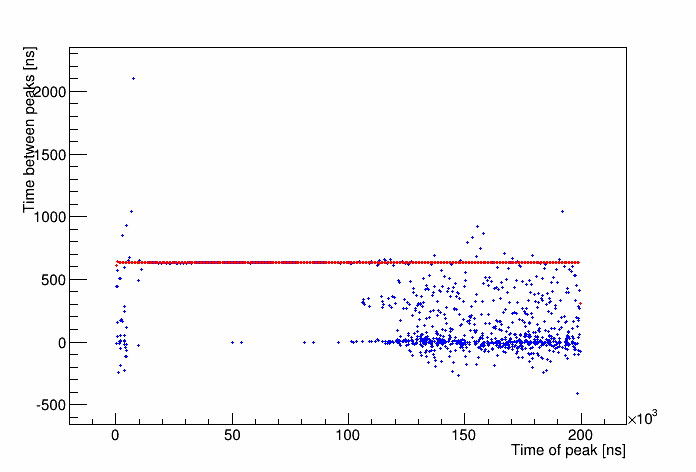
\includegraphics[width=\textwidth]{images/V=1_03_peak_deltas}
		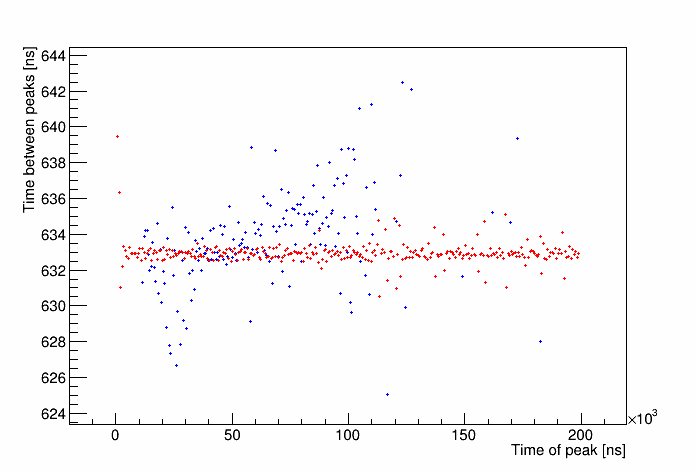
\includegraphics[width=\textwidth]{images/V=1_03_peak_deltas_zoom}
	\caption{Time between one peak and the next, for RF peak voltage of 0.5
           volts. (Top) the full trace (Bottom) the region around the RF
           period, 633 ns. The time between peaks for the RF pickup is shown in
           red, for the bunch monitor is shown in blue.}
	\label{fig:peak_deltas}
\end{figure}

\begin{figure}
	\centering
		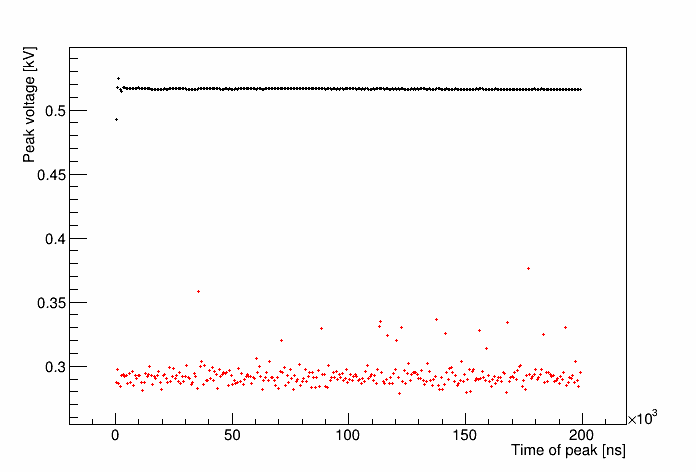
\includegraphics[width=\textwidth]{images/V=1_03_rf_voltage}
	\caption{The (black) RF voltage and (red) associated errors, magnified by
           $10^3$, for peak voltage of 0.5 volts.}
	\label{fig:rf_voltage}
\end{figure}

\begin{figure}
	\centering
		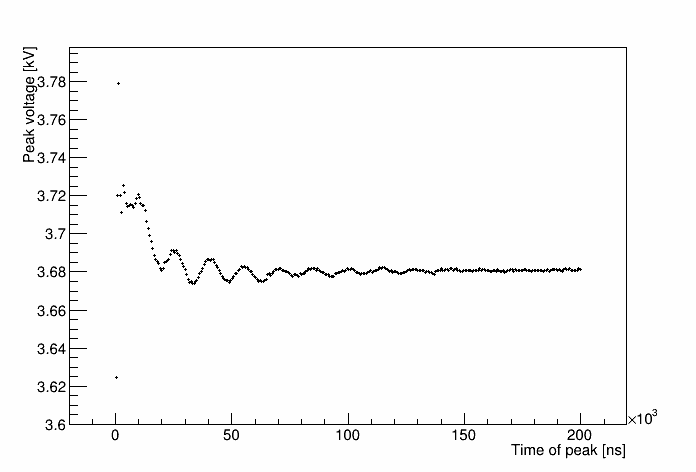
\includegraphics[width=\textwidth]{images/V=7_35_rf_voltage_zoom}
	\caption{The RF voltage for peak voltage 3.7 volts, showing ringing in
           the RF around injection.}
	\label{fig:rf_voltage_ringing}
\end{figure}

The magnitude and time of peaks and troughs was calculated using the peak 
finding algorithm outlined above. The time difference between adjacent peaks is
shown in Fig. \ref{fig:peak_deltas}. The frequency is seen to be stable across
many pulses, to within the measurement error. The oscillation magnitude, 
taken to be half the peak-to-trough difference, is shown in Fig. 
\ref{fig:rf_voltage}. This is stable for lower RF voltages but there is an 
oscillation at up to the 1$\%$ level at higher RF voltages (Fig. 
\ref{fig:rf_voltage_ringing}). This settles down
after of order a hundred microseconds, so one might imagine that adjusting the
ion source trigger could result in a more stable RF source.

The RF period is measured as 632.9 +/- 0.1 ns. The RF frequency is consistent at 
different voltages.

The measured RF voltages are listed below:
\begin{itemize}
\item 0.0001 +/- 0.00010
\item 0.1496 +/- 0.00009
\item 0.3801 +/- 0.00014
\item 0.5159 +/- 0.00010
\item 0.6874 +/- 0.00013
\item 0.7830 +/- 0.00021
\item 0.8924 +/- 0.00020
\item 1.1318 +/- 0.00021
\item 1.4166 +/- 0.00015
\item 2.3532 +/- 0.00034
\item 3.6822 +/- 0.00033
\end{itemize}
These voltages were calculated by taking half the average peak to trough 
distance of the last 10 peaks, in order to reject any initial instability as
discussed above. The stated error is the standard deviation of these values, and
is reasonably consistent with the calculated errors from fitting. The 
calibration between the measured voltage on the oscilloscope and the voltage in 
the cavity is 1 kV (error?). The statistical noise in the peak values is 
compatible with the error derived from the fitting routine described above.

\subsection{Bunch Monitor Signal}
The bunch monitor signal for S12 was read out to an oscilloscope where the data
was recorded.

For higher RF voltages, the beam is well captured and the peak-to-peak period is
roughly constant across a reasonable range. For lower voltages the beam is less 
well captured and the peak-to-peak period shows much greater variation. Even for 
the case where the beam is well captured, the spread in peak-to-peak times is 
larger than the calculated error in the peak finder, indicating that there may 
be some debunching or other behaviour occurring.

\section{Analysis}
There follows some analysis of the data.

\begin{figure}
	\centering
		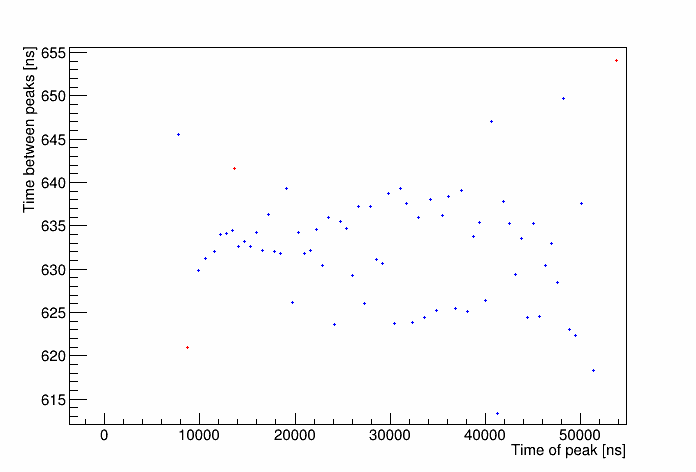
\includegraphics[width=\textwidth]{images/V=0_0_peak_deltas_zoom}
	\caption{Measured time of flight of the bunch around the ring in the absence
           of RF.}
	\label{fig:ring_time_of_flight}
\end{figure}


\subsection{Ring time-of-flight}
The ring time-of-flight can be measured directly using data taken with the RF
voltage set to 0. The ion source pulse was set to run over several cycles
of the RF. As the pulse length is not an exact multiple of the ring time of flight
so the final part of the pulse contributes an increase in the beam current which
mimics the behaviour of a beam pulse for the beam monitors, which operate in a
pulsed mode.

The relevant data and associated errors is shown in Fig. 
\ref{fig:ring_time_of_flight}. The ring time-of-flight is measured around 634 ns. It
is noted that the spread in measured time-of-flight values is larger than the
calculated measurement error on each peak would suggest, and grows rapidly over
the first 50 $\mu$s of the spill.

Despite this measurement uncertainty, the RF frequency seems to be quite 
compatible with the ring time-of-flight. The RF bucket length would have to be
less than the spread in measured time-of-flights, which is initially around 1 
ns, for incorrect frequency of the RF to be a significant contribution to
errors.

\begin{figure}
	\centering
		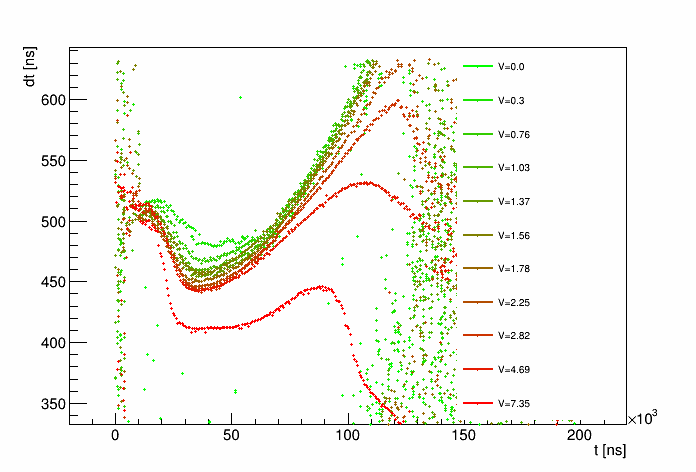
\includegraphics[width=\textwidth]{images/bpm_to_rf_deltas}
		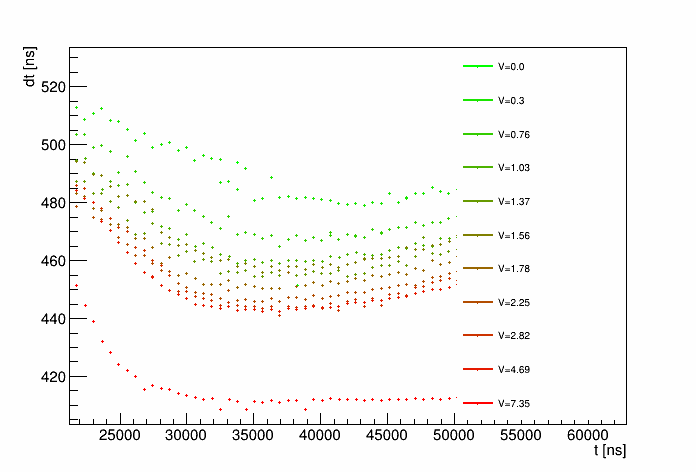
\includegraphics[width=\textwidth]{images/bpm_to_rf_deltas_zoom}
	\caption{Time difference between RF peak and any subsequent Beam monitor peaks
           as a function of time in the pulse. (Top) signal for the full pulse
           (Bottom) region used for calculating synchronous phase.}
	\label{fig:delta_rf_vs_bpm}
\end{figure}

\subsection{Time Difference Between RF Peaks and Bunch Monitor Peaks}
\emph{Dynamics is not simple and this section needs more thought.}

The principle aim of the analysis is to measure the time difference between the
RF peaks and the bunch monitor peaks. The time of Bunch Monitor peaks relative
to the immediately preceding RF peak is shown in Fig. \ref{fig:delta_rf_vs_bpm}.
Several regions are apparent. 

The beam is injected between 4 and 11 $\mu$s after
the initial trigger. As discussed above, the ion source pulse has an intrinsic 
bunch-like behaviour due to overlap of the start-of-pulse with the end-of-pulse 
in the ring. This pulse is not synchronised with the RF and so is not expected to be
captured in the bucket. It is washed out during the subsequent 10-20 $\mu$s and
subsequently the beam captured in the RF bucket is considered to be the dominant
signal.

After about 40 $\mu$s the bunch phase relative to the RF changes quite rapidly.
The beam is moving later in the RF signal, corresponding to a more accelerating
RF phase, indicating that the beam is losing more energy?

\subsection{Relative Phase Compared to RF Voltage}
In order to calculate a measured thickness of the foil, the RF phase is compared
to the peak voltage. For this study, the minimum time difference in the 30 
$\mu$s to 40 $\mu$s region is taken to represent the phase difference between 
the RF and the beam.

\begin{figure}
	\centering
		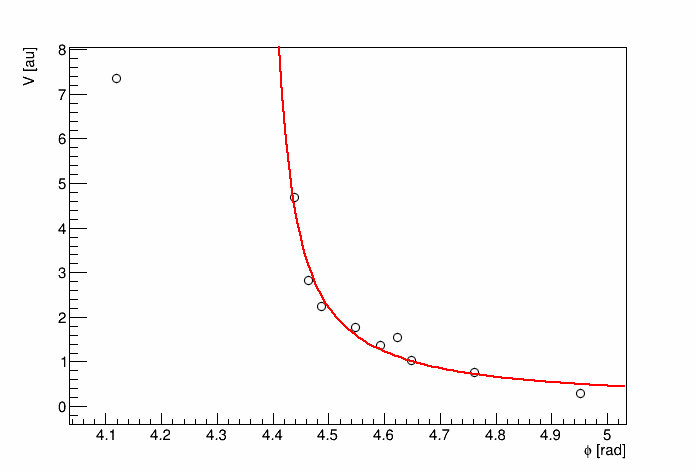
\includegraphics[width=\textwidth]{images/synchronous_phase_vs_voltage_cut}
		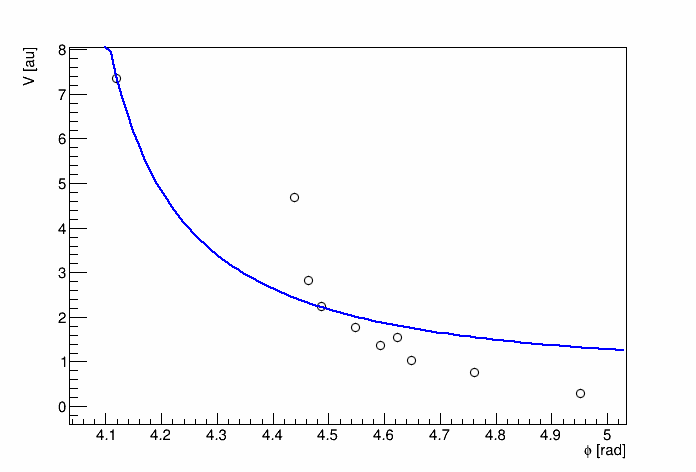
\includegraphics[width=\textwidth]{images/synchronous_phase_vs_voltage_unweighted}
	\caption{Measured synchronous phase compared with measured RF voltage. A fit .}
	\label{fig:synchronous_phase_vs_voltage}
\end{figure}


The relative phase difference is compared with the RF voltage in Fig. 
\ref{fig:synchronous_phase_vs_voltage}. Two figures are shown, in the first
instance the data is fitted against the full measurements, and in the second
instance the high voltage datum is excluded. There is no good reason to exclude 
the high voltage point except that it makes the fit much better. The fit 
function is

\begin{equation}
V_0 = dW/sin(\phi_s+d\phi).
\end{equation}

$d\phi$ is a calibration constant representing azimuthal offset of the RF
cavity and the bunch monitor, cable lengths and any associated electronics 
signal delays; $dW$ is the energy loss in the foil; $V_0$ is the measured 
voltage; and $\phi_s$ is the measured phase difference.

The calculated fit parameters for the two cases are listed below.
\begin{itemize}
\item High V case included: $dW = -1.10 +- 0.24$
\item High V case included: $d\phi = -0.829 +-   0.04 $    
\item High V case excluded: $dW = -0.270 +- 0.03 $
\item High V case excluded: $d\phi = -1.237 +-   0.009$    
\end{itemize}

It is noted that the fit quality and parameters are \emph{not} stable against
the region that is considered in the analysis. As the raw minimum of 
statistically fluctuating quantities is used, outliers may well be pulling the 
fit.

\section{Discussion}
Several questions remain open:
\begin{itemize}
\item Why does the phase change so drastically after 40$\mu$s?
\item Is there a bad data point in the higher voltage region? The 1$\%$ 
oscillation in RF voltage is noted but not expected to produce a strong effect.
Fitting to the minimum in Fig. \ref{fig:synchronous_phase_vs_voltage} would
be better, but it is necessary to understand the general shape of this figure
before really thinking too hard about any conclusions drawn from it.
\end{itemize}

\end{document}

